\documentclass{pelagicore}

\begin{document}
\title {GENIVI Browser}
\subtitle {Proof of Concept}
\revision{0.4}
\revisiondate{\today}
\author{Marcel Schuette, Pelagicore}
\lang{EN}
\approvedby{Marcel Schuette}
\location{Munich, Germany}
\filename{\jobname}
\docnumber{1}
\frontlogofile{genivi.png}
\bannerlogofile{genivi_small.eps}
\bannerlogoheight{0.5in}
\usefrontmetadatatrue
\company{GENIVI}

\maketitle
\tableofcontents \clearpage

\hyphenation{Webkit}

\section{Introduction and project background}
The GENIVI Networking Expert Group (NW-EG) would like to exercise a D-Bus-based
software component to test the usability and quality of a web browser that uses
the D-Bus interface. Therefore the expert group instructed a browser
Proof-of-Concept (PoC) to be executed to evaluate existing APIs and concepts.

\section{Scope of this document}

This document should give an overview about the architecture of the GENIVI
Browser PoC and details about the various components and their implementation.
With that document, it should be possible to understand the source code more
easily and get a better understanding of the used concept. Nevertheless the
document doesn’t replace reading the source code.

\section{Requirements}

The NW-EG defined a set of D-Bus APIs between the browser application and the
HMI.  These D-Bus APIs were provided as XML files. In addition, a header with
definitions of specific types and structures were provided prior to project
start.
\\\\
The NW-EG defined the following requirements:

\subsection{General Requirements}
\begin{tabularx}{\textwidth}{| p{4em} | p{6.5em} | X |}
    \hline
    \rowcolor{blue}
    \bf ID & \bf Requirement & \bf Description \\
    \hline
    SW-BRW-POC-001 & Environment   & The proof of concept must run under Ubuntu
                                     Linux 12.04 in a Virtual Box virtual
                                     machine installed on a desktop PC. \\
    \hline
    SW-BRW-POC-002 & Environment   & The implementation of the browser PoC will
                                     be done using the Qt 5 package which is
                                     under the LGPL v2.1 license. \\
    \hline
    SW-BRW-POC-003 & Documentation & Documentation describing how to install
                                     the software and run a set of acceptance
                                     tests shall be provided \\
    \hline
\end{tabularx}

\subsection{Architecture}
\begin{tabularx}{\textwidth}{|p{4em} | p{6.5em} | X |}
    \hline
    \rowcolor{blue}
    \bf ID & \bf Requirement & \bf Description \\
    \hline
    SW-BRW-POC-004 & Separation of Browser HMI and Browser-Core &
        The Browser shall be separated in HMI and Browser Core.
        A provided Qt-based test-HMI will control the Browser Core. \\
    \hline
    SW-BRW-POC-005 & Test-HMI as Separate Process &
        The provided test-HMI application will run as an independent process.\\
    \hline
    SW-BRW-POC-006 & Qt Webkit 1 implementation &
        The Browser PoC application must use the Qt5 Webkit1 implementation.\\
    \hline
    SW-BRW-POC-007 & QtWebview &
        The Browser POC must use QGraphicsWebView instead of QML webview.\\
    \hline
\end{tabularx}

\subsection{Browser Interfaces}
\begin{tabularx}{\textwidth}{|p{4em} | p{6.5em} | X |}
    \hline
    \rowcolor{blue}
    \bf ID & \bf Requirement & \bf Description \\
    \hline
    SW-BRW-POC-008 & D-Bus API & The Browser PoC shall implement the specified
                                 APIs as handed over in xml-form (see
                                 interfaces section)\\
    \hline
    SW-BRW-POC-009 & Qt Webkit Bridge & The Qt Webkit bridge should be useable
                                        in the Browser POC \\
    \hline
    SW-BRW-POC-010 & Netscape Plugin API (NPAPI) &
        The Browser POC should support the Netscape Plugin API (NPAPI) \\
    \hline
    SW-BRW-POC-011 & Configuration & The browser POC should implement a basic
                                     configuration mechanism for the browser\\
    \hline
\end{tabularx}

\subsection{Interfaces}
The following D-Bus interfaces files were provided as input to the project:

\begin{enumerate}
    \item IBookmarkManager.xml
    \item IBrowser.xml
    \item ICacheManager.xml
    \item IErrorLogger.xml
    \item INetworkManager.xml
    \item IUserInput.xml
    \item IWebPageWindow.xml
\end{enumerate}

These interfaces represent a subset of the GENIVI APIs defined by NW-EG and
contains only methods and signals, which has to be supported by the PoC. The
XML files can be found in the repository
(\url{http://git.projects.genivi.org/browser-poc.git/}) in the folder {\tt
/common}. For detailed information about the methods and signals for D-Bus
interfaces were defined, you can have a look at the files in the repository.

\section{Overview}
Following the requirements, the GENIVI Browser PoC is implemented with Qt 5 and
Qt Webkit 1. Although existing projects like the snowshoe browser were taken
into account, a `from scratch' approach was chosen. The specific requirements
of the project made a re-use of an existing project not appropriate, as a
reduction of efforts was not expected.
\\\\
The GENIVI Browser PoC consists of following components, which are also represented in
separate folders in the repository:

\begin{itemize}
    \item A browser application
    \item A test user-interface application (testUI)
    \item A demo user-interface application (demoUI)
    \item A set of automated tests ({\tt browser/unit-tests/*})
    \item A folder with common components
\end{itemize}

According to the defined architecture the browser application, which is
responsible for web page rendering and bookmark management, is separated from
the HMI (represented by the demoUI application and the testUI application). For
more detailed information about the architecture defined by NW-EG, you can have
a look at the group's wiki page
(\url{https://collab.genivi.org/wiki/display/genivi/Networking+Expert+Group}).

For instructions, how to build all applications or only a single application,
refer to the file {\tt BUILDINSTRUCTIONS}.

\section {Common part}
here is a common part in the project, which contains files, which are shared by
all applications. This common part is represented in the repository in the
folder {\tt /common}:

\begin{itemize}
    \item The XML files describing the interfaces
    \item A class defining a bookmark object (bookmark.h and bookmark.cpp)
    \item A class defining the D-Bus interfaces on client side (demoUI and test
          application) (browserdbus.h and browserdbus.cpp)
    \item A header file defining common types and structures (browserdefs.h)
\end{itemize}

The XML files are used to automatically generate the interface classes for
client and server. Via the generated interfaces of these classes, the clients
can call remote objects in the server via D-Bus.

\section{Browser Application}
\subsection{Introduction}
The Browser application is the core part of the PoC. It is responsible for
rendering and displaying a webpage with the QML webview element. It also
implements the defined server side interfaces for \texttt{IBrowser}, {\tt IUserInput},
{\tt IWebPageWindow}, {\tt ICacheManager}, {\tt IErrorLogger}, {\tt INetworkManager} and {\tt IBookmarkManager}. The bookmark manager includes also
logic for persistent bookmark storage in the system.

\subsection{Usage}
The browser application always needs to be started before the user-interface
application (demoUI or testUI) is started, because it creates the D-Bus
connection. As the window will be created by the user-interface application, no
window is shown at application start.  You can add an instance id as parameter
to the application start, e.g. {\tt ./browser 23}. The instance id will be
added to D-Bus service name, e.g. {\tt genivi.poc.browser23}. If no parameter
is given, a default instance id 1 is used.

\subsection{Structure}
The source code of the browser application can to be found in the {\tt
/browser} folder in the repository:
\\\\
\begin{tabular}{l l}
    *.cpp, *.h         & source and header files \\
    browser.pro        & Qt project file
\end{tabular}

\subsection{Implementation}
The browser application is implemented using QGraphicsWebView and Qt Webkit 1.

There is one class available for each defined interface group (XML file)
implementing the functions for the defined interfaces on server side. These
functions interact with the interfaces provided by the QML file.

As a central class the browserhelper class creates the connection to D-Bus on
the session bus and registers a service name on the D-Bus server. The default
service name for the GENIVI browser PoC is {\tt genivi.poc.browser + instance
id}, e.g. {\tt genivi.poc.browser23}. The default instance id is 1, if no
parameter is given, or the parameter given at application start.

The class also creates all interface objects and D-Bus interface adaptors,
registers needed types with the D-Bus system and registers the browser and
bookmark interface class with the D-Bus connection under an object path
(/Browser/IBrowser and /Browser/IBookmarkManager). The interface for
webpagewindow and userinput will be registered, when a new page is actually
created.

Each class is implemented in one header file and one cpp file, with the
extensions .h and .cpp respectively. Each .cpp file mentioned below also has an
associated .h file containing the class definition.

bookmarkmanager.cpp implements the IBookmarkManager interfaces and manages
persistent storage of bookmarks.

userinput.cpp implements the IUserInput interfaces.

browser.cpp implements the IBrowser interfaces, creates and set up a
declarative view with the main QML file (the webview) and registers
webpagewindow and userinput objects under a unique object path
(/Browser/IWebPageWindow + window handle resp. \\/Browser/IWebPageWindow + window
handle/IUserInput). This is needed to control different webpages or tabs
(created by the createPageWindow interface) with the testUI application. That
means e.g. routing a reload command to the right webpage window.

browserconfig.cpp handles persistant storage of configuration values and
provides a singleton for any part of the browser to access and set these
values.

browserpage.cpp is a subclass of QWebPage allowing BrowserView to intercept
dialog boxes and prompts.

cachemanager.cpp handles caching policies using {\tt
QNetworkConnectionManager}.

errorlogger.cpp handles error logging to an in-memory storage, and allows
D-Bus clients to query the error log.

browser/unit-tests/ contains the following: {\tt browserdbus} for D-Bus tests
of the browser and sub-components (webpageview, browserview, browserpage, etc),
{\tt browserview} for non-D-Bus tests of the broweserview, {\tt
cachemanagerdbus} and {\tt errorloggerdbus} for D-bus tests of {\tt
cachemanager} and {\tt errorloggerdbus} respectively.

\section{Test Application}
\subsection{Introduction}
With the test user-interface application, you are able to test all implemented
interfaces with all defined parameters. For this purpose, not the UI design of
the application was the key requirement, but the possibility to test the
functionality. This test application was also used to do manual tests, which
resulted in a test report
(\url{https://collab.genivi.org/wiki/display/genivi/Browser+Proof-Of-Concept+-
+Web+content#BrowserProof-Of-Concept-Webcontent-Testreport}).

\begin{figure}[!ht]
    \center
    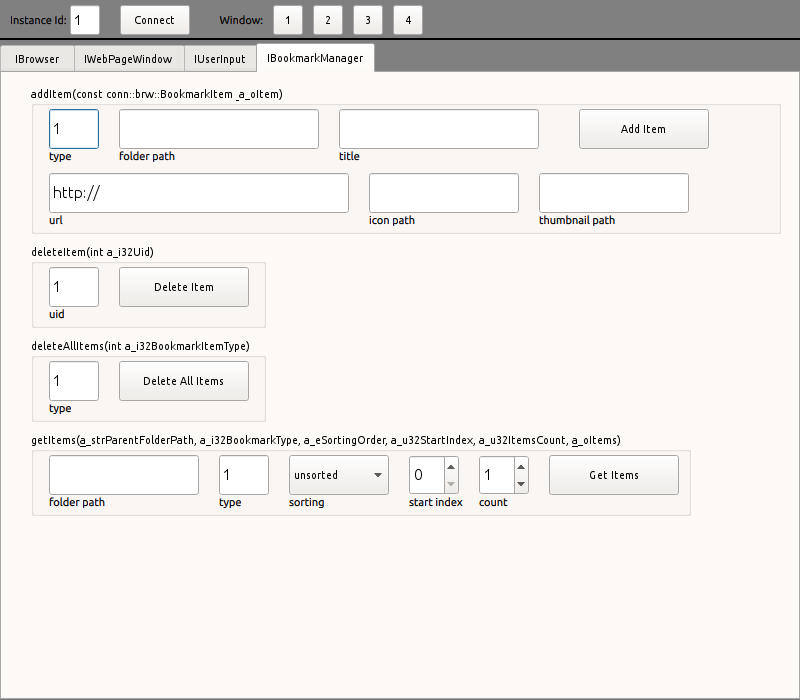
\includegraphics[width=0.8\textwidth]{testui.png}
    \caption{The picture above shows the testUI application with the bookmark
             manager tab visible.}
\end{figure}

\subsection{Usage}
Before the testUI application is started, the browser application must be
started. At startup only the bar on the top is visible, not the tabs or
buttons. First the testUI must connect to the D-Bus service. Therefore add the
correct instance id and press the connect button. The instance id is defined
with the browser application start, either 1 as default or the number given as
parameter at browser start.

The testUI application shows tabs representing the six interface groups
({\tt IBook\-mark\-Manager}, {\tt IBrowser}, {\tt IUserInput}, {\tt
IWebPageWindow}, {\tt ICacheManager} and {\tt IErrorLogger}). To navigate
between the groups, just press on the tab header.

On each page (or tab) each defined interface with its parameter is visually
grouped within a small frame. Each group consists of a button and optional
input fields, spin boxes or combo boxes, depending on the definition of the
parameters. By pressing the button of a group, the client calls a D-Bus
interface with given parameters, which calls a remote object on the server
side.

To be able to handle more than one opened window (e.g. redirect a press on the
reload button to the right window) with the testUI application, four buttons
(numbered from 1 to 4) were added to the bar on the top. For simplicity reasons
the buttons are limited to four, means only four windows can be managed with
the testUI application. The numbers on the buttons refer to the sequence the
windows were opened. E.g., if you want to reload the third opened window, first
press button 3 and then the reload button on the IWebPageWindow tab.

\subsection{Structure}
The source code of the test user-interface application can to be found in the
{\tt /testapp} folder in the repository:
\\\\
\begin{tabularx}{0.9\textwidth}{l X}
    main.cpp            & mainsource file \\
    testapp.pro         & Qt project file \\
    {\tt qml/testapp/*} & QML files for user interface \\
    {\tt images/*}      & Images used in implementation (icons taken from KDE
                          oxygen theme 4.10.3)
\end{tabularx}
\\\\

\subsection{Implementation}
The testUI application supports all interfaces described in the XML files.

The testUI application is implemented as a Qt Quick 2 application. The
user-interface is described with QML using Qt Quick Controls (reusable UI
controls provided by Qt 5.1).  Besides the main.QML file, which describes the
main view with all tabs, each interface group is described in a separate QML
file. The backend logic of the testUI application is written in C++. The main
task of the C++ part is to set up the view for QML, load the QML file and
register custom C++ type in the QML system (bookmark and browserdbus classes).
The browserdbus class represents the D-Bus interface for the client. It creates
the D-Bus channel connections, registers custom types with the QtDBustype system
and defines and calls all D-Bus interfaces and handles the return values. The
output of all return values, resulting from D-Bus remote object calls, is logged
onto the console.

\section{Automated tests}
The projects ships with an automated test suite, located under {\tt
browser/unit-tests}. The tests are divided into different sub-groups, each
placed in its own directory. The test directories ending with "dbus"
communicate with the browser over D-Bus.

The {\tt browserdbus} directry contains tests for the {\tt browser} component
and sub-components. These tests will interact with a Webkit surface using mouse
and keyboard input over D-Bus. For mouse input, the {\tt
xdotool}\footnote{http://www.semicomplete.com/projects/xdotool/} is used, and
this tool is required to be installed in {\tt \$PATH} run these tests. These
tests also require the actual browser to be running.

The {\tt browserview} directory contains tests of the {\tt browserview}
component, these tests do not run over D-Bus.

The {\tt cachemanagerdbus} directory contains D-Bus tests for the {\tt
cachemanager}. These tests require the browser to be running.

The {\tt errorloggerdbus} directory contains D-Bus tests for the error logger
component. The tests will launch the neccessary browser components itself, and
does not require the browser to be running. The tests will use the same D-Bus
name space as the browser component, so running the browser during these tests
will result in an error.

\section{Demo User-Interface}
\subsection {Introduction}
The idea of the demo user-interface application is to have a user-interface,
which looks more like a possible real browser user-interface (other than the
testUI application) and can be used to demonstrate the GENIVI Browser PoC at
shows and events. The demoUI application doesn’t support the full set of
defined interfaces, but only a subset needed to demonstrate the used features.
The chosen features were selected to be the main features known from common web
browsers.

\begin{figure}[!ht]
    \center
    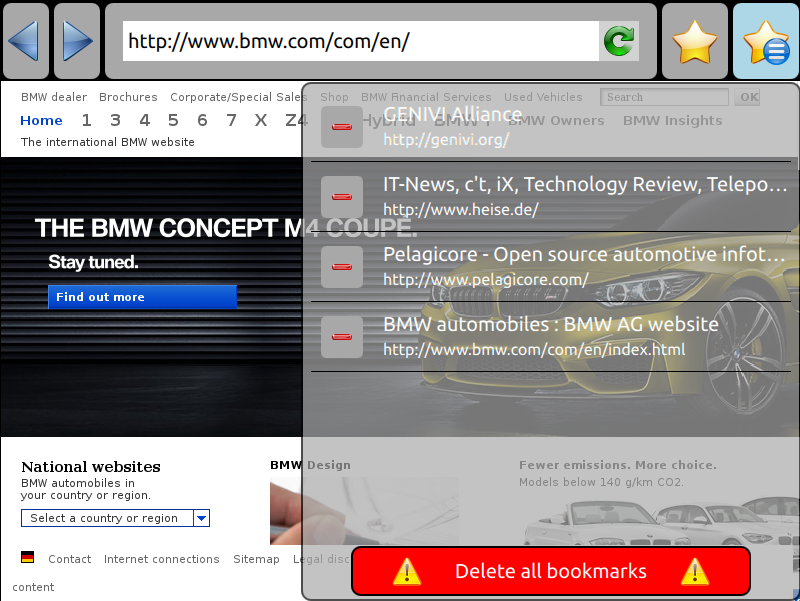
\includegraphics[width=0.8\textwidth]{demoui.png}
    \caption{The picture above shows the demo user-interface application with
             open bookmarks pane. The website shown in the background is part
             of the browser application.}
\end{figure}

The demoUI supports the following features:
\begin{itemize}
    \item loading a web page defined by a URL
    \item bookmark management (add, select, delete and delete all bookmarks)
    \item navigation back and forward in the browser history
    \item reload and stop loading a web page
    \item display a progress bar representing the loading progress of a web page
          (displayed below the URL in the input field)
    \item keypad navigation on web page with keyboard navigation keys
\end{itemize}

\subsection{Usage}
Before the demoUI application is started, the browser application must be
started. With the start of the demoUI application, also the browser application
becomes visible. The two applications (browser and demoUI) are arranged in a
seamless way, to represent the look of only one application.

The icons in the demoUI are hopefully self-explaining and known from other web
browser user-interfaces. To load an URL type the URL in the input field on the
top and press the enter key on an attached keyboard. The two top-right icons
represent `add bookmark to bookmark list' and `show bookmark list'
functionality. If the bookmark pane is open, you can select bookmarks to be
loaded in the webview, delete individual bookmarks by pressing the red `minus'
icon at the front of a bookmark or delete all bookmarks with the red button on
the bottom of the pane. For keypad navigation on webpages, the up-, down-,
right- or left-key (line mode) or the space bar (page down) and tab key (page
up) (page mode) can be pressed. It's important that the demoUI application has
the focus to receive the key presses. To activate a link on a web page or move
the web page, the browser application window can be directly accessed. These
actions are not handled over a D-Bus interface.

\subsection{Structure}
The source code of the demo user-interface application can to be found in the
{\tt /demoui} folder in the repository:
\\\\
\begin{tabularx}{0.9\textwidth}{l X}
    main.cpp                    & mainsource file \\
    demoui.pro                  & Qt project file \\
    {\tt qml/demoui/*}          & QML files for user interface \\
    {\tt qtquick2application/*} & Classes for displaying a QtQuick UI \\
    {\tt images/*}              & Images used in implementation (icons taken
                                  from KDE oxygen theme 4.10.3)
\end{tabularx}
\\\\

\subsection{Implementation}
The demoUI supports the following D-Bus interfaces:
\begin{itemize}
    \item IBrowser
    \begin{itemize}
        \item createPageWindow (with fixed parameters)
    \end{itemize}
    \item IWebPageWindow
    \begin{itemize}
        \item load
        \item reload
        \item stop
        \item back
        \item forward
        \item scroll (line or page scrolling)
        \item onLoadStarted
        \item onLoadProgress
        \item onLoadFinished
    \end{itemize}
    \item IBookmarkManager
    \begin{itemize}
        \item addItem (with url and title, all other parameter fix)
        \item getItems (with fixed parameters)
        \item deleteItem
        \item deleteAllItems (with fixed parameters)
    \end{itemize}
\end{itemize}

The demoUI is implemented as Qt Quick 2 application. The user-interface is
described with QML. The backend logic of the demoUI is done in C++. Main task
of the C++ part is to set up the view for QML, load the QML file, register
custom C++ type in the QML system (bookmark and browserdbus classes). The
browserdbus class represents the D-Bus interface for the client. It creates the
D-Bus channel connections, registers custom types with the QtDBustype system
and defines and calls all D-Bus interfaces and handles the return values. The
output of all return values, resulting from D-Bus remote object calls, is logged
onto the console.

If the bookmark pane is open, the demoUI application (geometry) is resized. The
height of the application is changed. This resize is needed, to show the pane,
which has the height of the complete browser, and to allow (if closed) getting
access to the browser window (e.g. pressing on links on the browser window).
Otherwise the above lying application with the focus (even if parts of the
application are transparent) would get all mouse and key events and it wouldn’t
be possible to click on links on a web page.

\end{document}
